\documentclass[a4paper, 11pt]{article}

\setcounter{tocdepth}{3}
\setcounter{secnumdepth}{3}

\usepackage{comment} % enables the use of multi-line comments (\ifx \fi) 
\usepackage{lipsum} %This package just generates Lorem Ipsum filler text. 
\usepackage{fullpage} % changes the margin
\usepackage[utf8]{inputenc}
\usepackage{gensymb}
\usepackage{graphicx}
\usepackage{booktabs}% http://ctan.org/pkg/booktabs
\usepackage{makecell}
\usepackage{tabularx}
\usepackage[table]{xcolor}
\usepackage{array}
\usepackage{wrapfig}
\usepackage{subcaption}
\usepackage{csquotes}
\usepackage{lscape}
\usepackage{afterpage}
\usepackage{geometry}
\usepackage{listings}

\geometry{a4paper, margin=1in}
\renewcommand{\figurename}{Abb.}

\begin{document}
\title{Zusammenfassung Future IT-Infrastructure FS2018}
\author{Alex Neher}
\maketitle

\tableofcontents
\newpage

\graphicspath{{./Pictures/}}

\section{Netzwerk-Aspekte}
\subsection{VPN}
Ein VPN (Virtual Private Network) erlaubt es einem Benutzer, sich in ein Netzwerk 'einzuklinken', selbst wenn er physisch nicht am Standort des Netzwerks ist.

\subsubsection{Szenarien}
Es gibt verschiedenste Szenarien, in welchen ein VPN nützlich oder vonnöten ist. Einige davon sind z.B:
\begin{description}
	\item [Remote Access: ] Management eines Kundennetzwerks vom (Home-)Office aus, Zugriff auf HSLU-Ressourcen von zuhause. US-Netflix in der Schweiz schauen
	\item[Site-to-Site VPN: ] Verbindung zweier Netzwerke über einen verschlüsselten Tunnel. Von der Azure-Cloud ins EnterpriseLab, Verbindung zwischen zwei fixen IPs.
\end{description}

\subsubsection{Technologien}
Es gibt verschiedene Technologien, wie ein VPN aufgebaut sind. die zwei wichtigsten sind:

\begin{description}
	\item[SSL-VPN] Wird vor allem für \textbf{Remote Access} verwendet, da es mit einem relativ einfachen Setup verbunden ist. SSL-VPN läuft ausschliesslich über \textbf{Port 443 (HTTPS)}
	\item[IPSec-VPN] Dieses Protokoll wurde ursprünglich exklusiv für IPv6 entwickelt, ist nun aber auch auf IPv4 portiert worden. Es kann, wie das SSL-VPN ebenfalls für Remote Access eingerichtet werden, ist jedoch auch nützlich für Site-to-Site VPNs. IPSec-VPN wird als \textbf{wichtigstes VPN-Protokoll} heutzutage angeschaut.
\end{description}

\noindent Des weiteren gibt es noch diese zwei, veralteten und unsicheren Protokolle, die jedoch immer noch eingesetzt werden.

\begin{description}
	\item[PPTP (Point-to-Point-Tunneling Protocol): ] Basiert auf PPP \footnote{Point-to-Pont-Protocol}, ist jedoch veraltet und unsicher.
	\item[L2TP (Layer 2 Tunneling Protocol): ] Ist unverschlüsselt und vertraut darauf, dass wichtige Daten verschlüsselt werden, bevor sie getunnelt werden. Dementsprechend veraltet und unsicher.
\end{description}

\newpage

\subsubsection{IPSec}

\begin{wrapfigure}[13]{L}{0.55\textwidth}
	\centering
	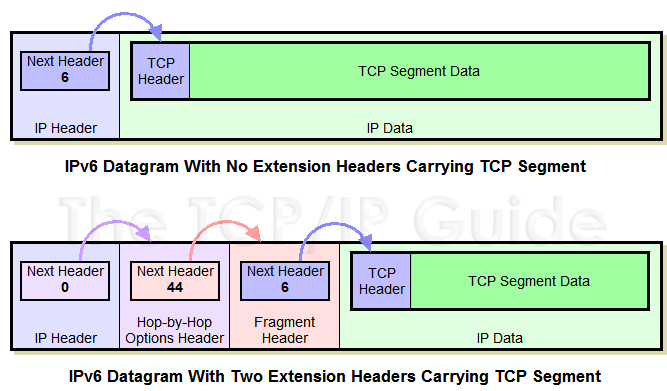
\includegraphics[keepaspectratio=true,height=10\baselineskip]{ipv6header.png}
	\caption{IPv6 unterstützt optionale Headers, die zwischen Payload und Header eingeschoben werden.}
	\label{fig:ipv6header}
\end{wrapfigure}


Da IPSec ursprünglich für IPv6 entwickelt wurde, unterstützt es dessen Konzept der \textbf{Header Extensions} (Abbildung \ref{fig:ipv6header}). IPv4 unterstützt jedoch \textit{keine} Header-Extensions! Bei IPv4 werden diese IPSec-Header einfach zwischen dem IP-Header und dem TCP/UDP-Header eingefügt.

\vspace{10px}

\noindent IPSec unterstützt die Verwendung des \textbf{AH} und/oder \textbf{ESP-Headers}.

\begin{description}
	\item[AH (Authentication Header): ] Die Authentizität des Datenursprungs ist sichergestellt.
	\item[ESP (Encapsulating Security Payload): ] Die Daten sind verschlüsselt
\end{description}

Die eingefügten Header beinhalten eingentlich nur eine \textbf{Sequenznummer} und einen \textbf{Index auf eine SA} (Security Association). Zudem wird das gesamte Paket noch mit einem \textbf{Hashwert} versehen, was jedoch dank NAT zu Problemen kommen kann, da das NAT die Authentizitäts-Garantie des Authentication Headers versaut.

\paragraph{Security Association} \mbox{} \\
Jedes IPSec Endgerät kann \textbf{beliebig viele} SA speichern. Eine SA ist grundsätzlich nur eine \textbf{Datenstruktur}, die (unter anderem) folgende Felder Informationen enthält:

\begin{description}
	\item[Authentifationsverfahren: ] Modi und Schlüssel falls AH verwendet wird.
	\item[Verschlüsselungsverfahren: ] Modi und Schlüssel, falls ESP verwendet wird.
	\item[Lebensdauer der SA und Schlüssel: ] Wie oft muss der VPN-Tunnel wiederhergestellt werden.
	\item[IP-Adresse der End-Netzwerk Gateways]
\end{description}

\noindent Beim Verbindungsaufwand wird diese SA aufgebaut. Dazu wird das \textbf{ISAKMP (Internet Security Association Key Management Protocol)} verwendet. 

\paragraph{ISAKMP}\mbox{} \\
 Das ISAKMP Protokoll besteht aus zwei Phasen:
\begin{description}
	\item[Phase 1: ] Ein \textbf{gemeinsamer Schlüssel} wird mit einem \textbf{erweiterten Diffie-Hellman-Verfahren} ausgehandelt (Bürgler lässt grüssen). Anschliessend werden die \textbf{Verschlüsselungs- und Hash-Protokolle ausgehandelt (nun in verschlüsselter Kommunikation)}. Dabei gibt es zwei verschiedene Modi: Im Main-Modus einigen sich beide Parteien auf die verwendeten Protokolle, während im Aggressiven Modus der Initiator 'seine' Protokolle vorgibt. Die Partner authentisieren sich via PSK, ihre Digitale Signatur, RSA oder El-Gamal.
	\item[Phase 2: ] Die SA wird nun aufgebaut und die weiteren Parameter für die IPSec-Verschlüsselung und den Tunnel werden ausgetauscht.
\end{description}

\newpage

\paragraph{Transport- vs. Tunnel-Mode}\mbox{} \\
\begin{wrapfigure}[16]{R}{0.6\textwidth}
	\centering
	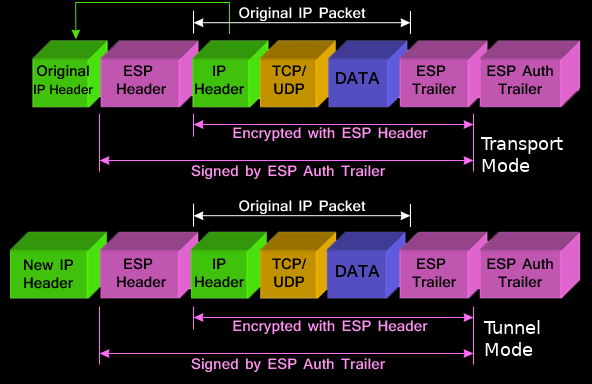
\includegraphics[keepaspectratio=true,height=12\baselineskip]{tunnelvstransport.png}
	\caption{Unterschied der Header zwischen dem Transport- und dem Tunnel-Mode}
	\label{fig:tunneltransport}
\end{wrapfigure}

Diese vorhin genannten weiteren Parameter sind z.B. ob der \textbf{Transport-} oder det \textbf{Tunnel-Modus} verwendet werden und ob \textbf{NAT-Traversal}\footnote{Ermöglicht es, das AH-NAT-Problem zu umgehen, indem die Pakete in UDP-Pakete encapsulated werden, die anschliessend über Port 4500 versendet werden..} erlaubt sein sollte.

Bei IPSec ist per Default der \textbf{Tunnel-Mode} eingestellt. In diesem Modus wird das \textbf{gesamte IP-Paket verschlüsselt}. IPSec nimmt es, verschlüsselt es, packt seinen IPSec Header davor und schickt es durch den Tunnel. Die allfälligen AH- und ESP-Header werden zwischen dem 'alten' IP-Header des zu verschlüsselnden Pakets und dem 'neuen' IP-Header des IPSec-Protokolls gepackt (Abbildung \ref{fig:tunneltransport} unten). 

Beim \textbf{Transport-Mode}, der hauptsächlich bei \textbf{End-to-End-Verbindungen)} wie z.B. Client zu Server eingesetzt wird, wird das IP-Paket durch \textbf{AH und/oder ESP-Header} verschlüsselt. Der IP-Header des Pakets wird beim Transport-Mode an den Anfang geschoben, gefolgt vom ESP (und evtl. AH-Header).

Transport-Mode wird meist mit einem anderen tunneling-Protokoll wie z.B. GRE gekoppelt. So wird der original Payload zuerst von GRP umschlossen, bevor IPSec das neue, umschlossene Paket durch den Tunnel schickt.

\paragraph{Verbindungsprobleme mit IPSec} \mbox{} \\
Es kann auch zu 'Show-Stopper' kommen beim Verbindungsaufbau mit IPSec, die verhindern, dass die Verbindung aufgebaut werden kann.

\begin{itemize}
	\item Der Initiator ist im Aggressiv-Mode und der Partner unterstützt die verlangten Protokolle oder den Aggressiv-Mode nicht (z.B. Android)
	\item Bei Remote Access VPN müssen IP-Adressen und weitere Informationen dynamisch übermittelst werden, die evtl. nicht untereinander kompatibel sind.
	\item Es gibt kein gemeinsames Set von Verschlüsselungs- oder Hash Algorithmen der beiden Seiten, bzw. die unterstützten Schlüssellängen sind nicht komptabiel.
\end{itemize}

In aller Regel sind Site-To-Site VPNs aber trotzdem möglich, solange die verwendeten Algorithmen bekannt und kompatibel sind.

\subsection{WAN-Technologien}
 

\section{Identity Management}

\section{Cloud Resources}

\section{Evalutation von Cloud-Services}

\section{Platform Trends}

\section{Betriebliche Aspekte}

\end{document}